% ============================================================
%  第5章  系统测试与结果分析
% ============================================================
\chapter{系统测试与结果分析}

本章从硬件性能验证、姿态解算精度评估、训练模式功能测试和系统整机稳定性测试四个方面，对头戴式眼部康复装置进行了全面的实验测试，并对测试结果进行了数据分析。测试中发现并解决了若干设计和调试过程中的技术问题。

\section{硬件测试}

\subsection{PWM波形验证}

SG90舵机所需的50Hz PWM信号由TIM1定时器生成，两个通道分别对应PE9（TIM1\_CH1，Y轴舵机）和PE13（TIM1\_CH3，X轴舵机）。测试采用数字示波器直接测量两个引脚的输出波形。舵机90°时pwm波示波器波形如图\ref{fig:pwm_wave}所示，波形稳定且无明显抖动，脉宽1500us。

\begin{figure}[h!]
\centering
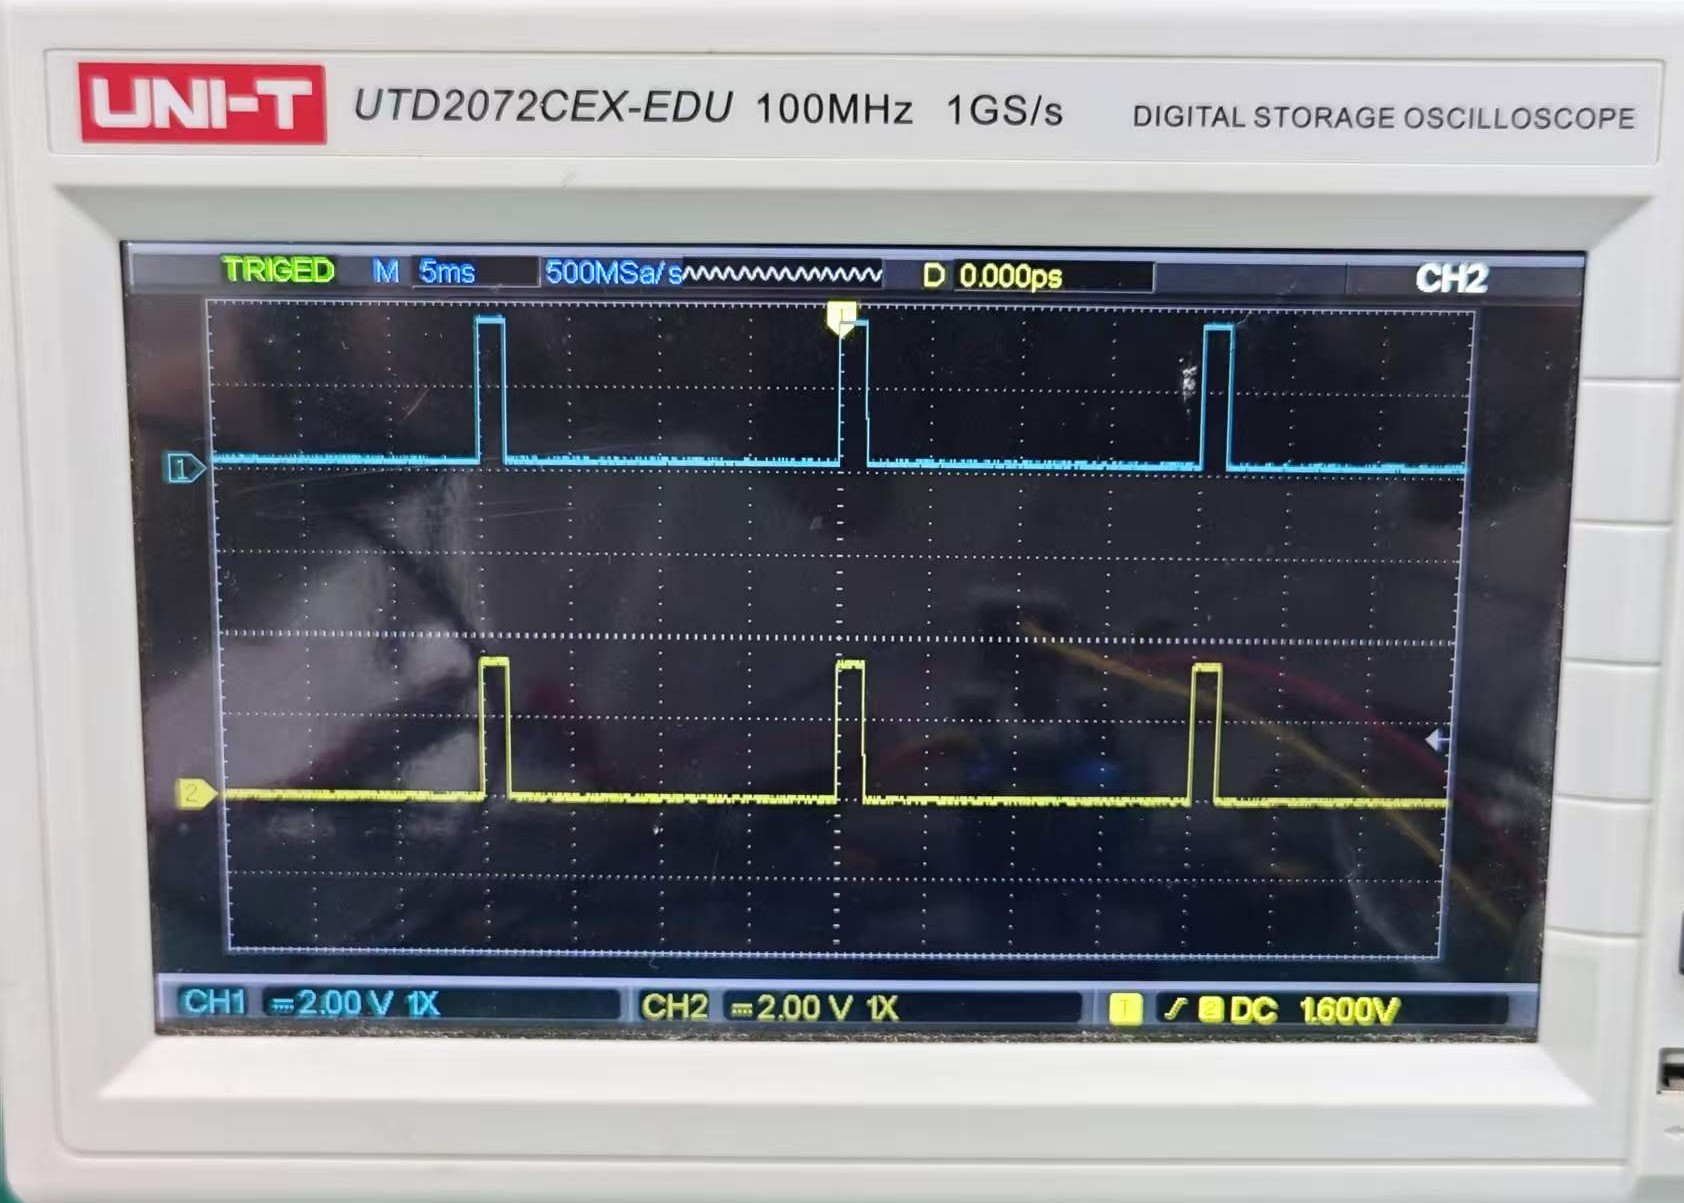
\includegraphics[width=0.85\textwidth]{figures/pwm_wave.jpg}
\caption{Y轴舵机(上)和X轴舵机(下)在90°角度下的PWM输出波形}
\label{fig:pwm_wave}
\end{figure}

首先验证PWM周期。50Hz对应的理论周期为20.0ms，实测PE9引脚周期约为19.98ms，PE13引脚约为20.01ms，均在可接受的误差范围内。随后使程序依次输出0°、45°、90°、135°和180°五个标称角度对应的PWM信号，测量各角度下的实际脉冲宽度，结果如表\ref{tab:pwm_test}所示。

\begin{table}[h!]
\centering
\caption{TIM1 PWM输出测试结果}
\label{tab:pwm_test}
\begin{tabular}{p{2.5cm} p{3cm} p{3cm} p{3cm}}
\toprule[1.5pt]
\textbf{舵机角度} & \textbf{理论脉宽 (us)} & \textbf{PE9实测脉宽 (us)} & \textbf{PE13实测脉宽 (us)} \\
\midrule[1pt]
0°   & 500  & 497  & 502  \\
45°  & 1000 & 1003 & 998  \\
90°  & 1500 & 1501 & 1500 \\
135° & 2000 & 1997 & 2004 \\
180° & 2500 & 2503 & 2495 \\
\bottomrule[1.5pt]
\end{tabular}
\end{table}

测试结果表明，实际脉宽与理论值的偏差控制在$\pm$5us以内，对应角度误差不超过0.5°，满足康复训练场景对舵机定位精度的要求。此外，验证了舵机从0°跳变至180°的过渡过程中PWM波形连续无中断，未出现脉冲丢失或尖峰信号。

蜂鸣器驱动方面，PB15（TIM12\_CH2）输出5kHz方波。当CCR2设置为0时蜂鸣器静音，设为500（对应约50\%占空比）时输出最大响度，与预期相符。

\subsection{语音模块UART通信测试}

语音模块通过UART7接口与STM32主控连接。测试分为发送验证和接收验证两个阶段。

发送测试中，将语音模块通过USB转串口适配器（CH340）连接至电脑，通过串口助手发送AA 55 FF 09 FB （“初始化完成”）协议帧，模块正确播报“初始化完成”；随后接收验证中，向模块说出“你好小盈”，模块播报“请吩咐”，并在串口助手上接收到AA 55 03 00 FB 协议帧，如图\ref{fig:uart_tx}所示，进一步验证了UART7接收通道的基本功能。

\begin{figure}[h!]
\centering
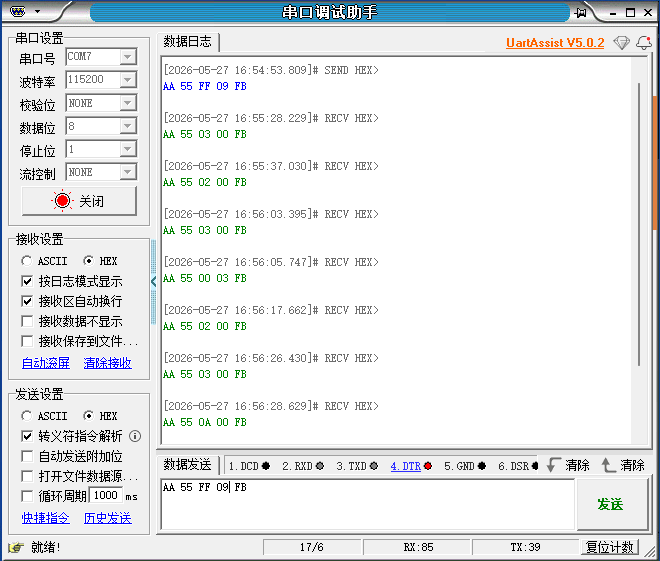
\includegraphics[width=0.8\textwidth]{figures/uart_tx.png}
\caption{串口助手捕获的UART7发送帧}
\label{fig:uart_tx}
\end{figure}


\section{姿态解算验证}

\subsection{静态零偏与噪声测试}

将装置平稳放置于水平桌面使BMI088传感器处于完全静止状态，上电完成800样本校准后连续采集10秒陀螺仪数据（约1000个采样点）。经零偏补偿后，三轴角速度的均值分别为X轴$-0.012$dps、Y轴$0.008$dps、Z轴$0.015$dps，均接近零值。三轴角速度的标准差分别为0.041dps、0.037dps和0.044dps，静态噪声水平约为0.04dps。该结果表明BMI088在静止条件下具有较低的固有噪声，800样本校准方案有效抑制了初始零偏。

\subsection{动态角度跟踪测试}

测试人员戴上装置，依次完成点头、左右转头、侧倾以及组合运动这四个标准动作，然后查看并记录下欧拉角的实时反应。以点头动为例，测试人员从正视前方慢慢低头到大约45度左右，在这个过程中pitch角处在0°附近的小范围波动(±2°)，而当其下降到接近−38°的时候，pitch角也随之随之减小到了差不多这个数值，并且在返回的过程中也是相当平稳的，并没有出现明显的抖动或者突变现象。转头动作中roll角保持了和实际转动角度一致的变化趋势，没有大的起伏或者跳跃式变化。点头、转头、侧倾运动下的IMU欧拉角跟踪曲线如图5-3所示，总体上具有较好的动态响应特性及稳定的姿态解算结果，红色曲线为roll角，绿色曲线为pitch角，蓝色曲线为yaw角。

需要注意的是，由于没有磁力计给出绝对地磁参考，所有的角度都是通过陀螺仪Z轴角速度积分来得到的。在静止状态下大约有0.5°的漂移现象，在一个训练时间段(15-50s)内，侧倾角的变化范围为1°到2°之间，可以满足训练时精度的要求。

\begin{figure}[h!]
\centering
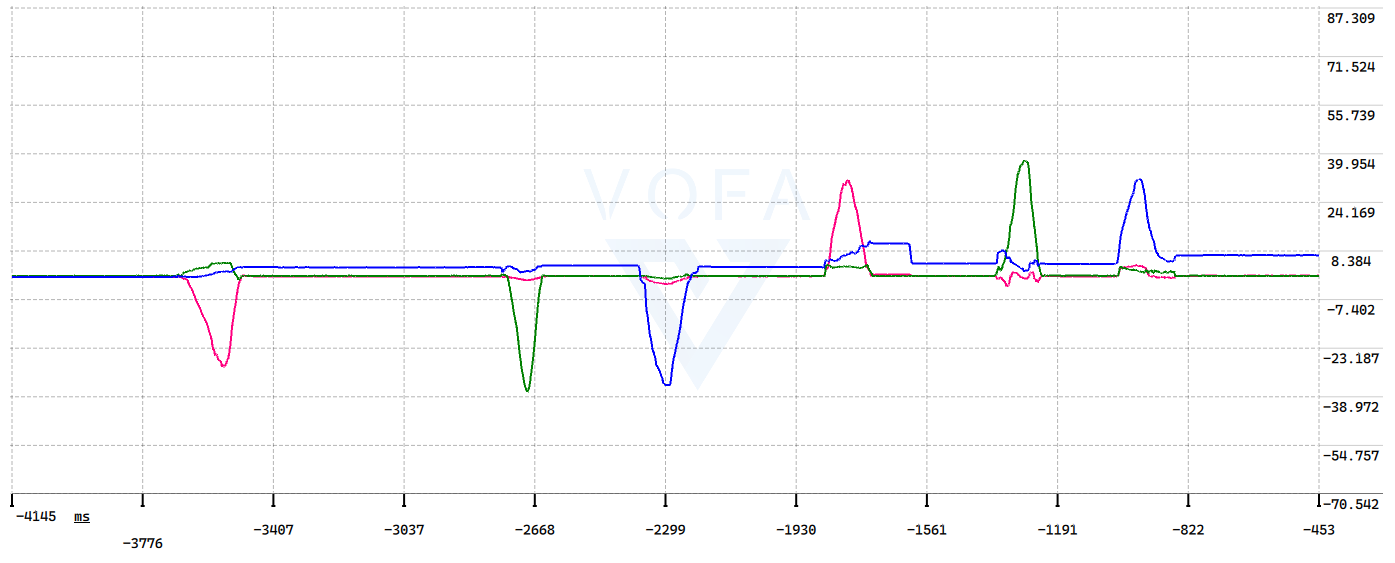
\includegraphics[width=1.0\textwidth]{figures/euler_track.png}
\caption{点头-转头-侧倾运动下三轴欧拉角变化曲线}
\label{fig:euler_track}
\end{figure}

\subsection{漂移测试}

为了评价长时间工作时各个欧拉角的累积误差，在静止状态上连续运行了5分钟，得到各个角的变化曲线。在5分钟的测试周期内，三个欧拉角都没有出现明显漂移，在±0.5°以内，这个漂移速度在一次训练时间（最长50s的视觉聚焦训练）里对于训练中姿态监测几乎没有影响。具体的曲线如下图5-4所示，红色为roll角、绿色为pitch角、蓝色为yaw角。

\begin{figure}[h!]
\centering
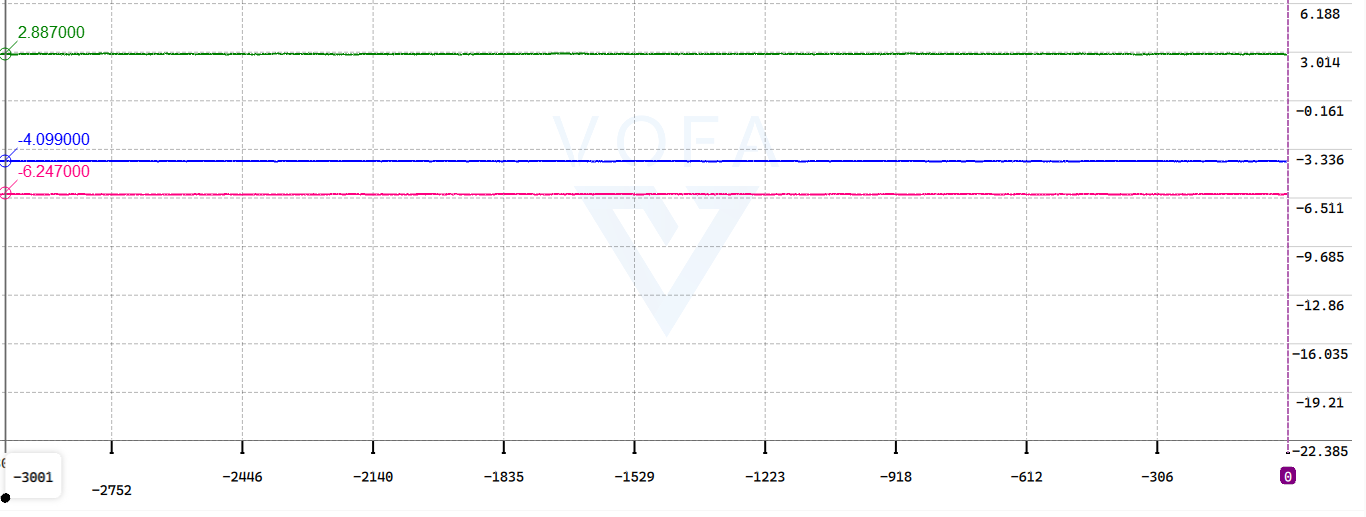
\includegraphics[width=1.0\textwidth]{figures/drift_test.png}
\caption{长时间运行条件下各欧拉角的漂移变化曲线}
\label{fig:drift_test}
\end{figure}

\section{训练模式功能验证}

\subsection{双模式选择与切换测试}

模式选择通过PA2按键的单击或者双击来区分，双击窗口设置为600ms。在测试过程中进行了五次单击和五次双击，单击全部正确进入完整的训练模式，双击全部正确进入自选模式，没有出现因为双击而误认为是两次单击或者单击而误认为是双击的情况。双击窗口阈值600ms对老年人的操作速度比较合适。

跨状态语音模式切换测试是在自选模式下进行的。使用语音命令进入到扫视训练状态，在训练执行的过程中，系统安全暂停时以及系统的反馈评价状态下都说了平稳追踪训练的话术，这表明该系统可以在一个调用状态机主运行函数周期内执行好模式的转变任务。三种情况的切换延迟均小于100ms，即立刻停止当前正在进行中的训练工作，开始陀螺仪校准并切换到新的模式下系统的训练提示状态，并没有任何卡顿出现。

\subsection{模式A：注视稳定性训练}

注视稳定性测试采用被试者端坐于仪器上，用固定的激光指向墙面15秒的方法进行。选取了三个不同头部稳定的受试者参加实验，在每个受试者的身上放置一个装置，并且让其一直注视着墙上的一条直线上的一个点。为了使结果更具有代表性，对每个受试者做了三次测量取平均数得到如表\ref{tab:fixation_test}所示的结果。

\begin{table}[h!]
\centering
\caption{注视稳定性训练测试结果（三次重复取平均）}
\label{tab:fixation_test}
\begin{tabular}{p{3.5cm} p{2.5cm} p{2.5cm} p{2.5cm}}
\toprule[1.5pt]
\textbf{受试者} & \textbf{稳定状态} & \textbf{平均头稳指标 (°)} & \textbf{语音提醒次数} \\
\midrule[1pt]
受试者A（正常） & 刻意保持静止   & 1.82  & 0 \\
受试者B（轻晃） & 自然微小晃动  & 4.53  & 3 \\
受试者C（强晃） & 故意大幅度摆动 & 8.31  & 7 \\
\bottomrule[1.5pt]
\end{tabular}
\end{table}

三组受试者头稳指标存在明显的分层，在保持静止状态下约为1.8°、自然微小晃动约为4.5°、大幅度摆动约为8.3°。系统会根据头稳指标来分层出不同的头部稳定程度，并且语音提示只会在头稳指标超过5°阈值的时候才会触发。

\subsection{模式B：扫视训练}

扫视训练在标定模式确定的视野四角点之间随机跳变，每轮8个试次，受试者看到激光光点后按PA2确认。对同一受试者进行了三轮重复测试，以观察学习效应，数据如表\ref{tab:saccade_test}所示。

\begin{table}[h!]
\centering
\caption{扫视训练测试结果}
\label{tab:saccade_test}
\begin{tabular}{p{1.5cm} p{2cm} p{1.6cm} p{2.2cm} p{2.5cm} p{2cm}}
\toprule[1.5pt]
\textbf{轮次} & \textbf{正确/总次数} & \textbf{正确率} & \textbf{平均反应时 (s)} & \textbf{连续正确触发} & \textbf{评价} \\
\midrule[1pt]
第1轮 & 6/8  & 75.0\%  & 2.31  & 否 & 表现不错 \\
第2轮 & 8/8  & 100.0\% & 1.67  & 是（4--6次）& 非常出色 \\
第3轮 & 8/8  & 100.0\% & 1.52  & 是（3--5次）& 非常出色 \\
\bottomrule[1.5pt]
\end{tabular}
\end{table}

第一轮测试中受试者还不知道操作方法，反应慢并且出现了两次超时。第二、第三轮正确率为100\%，平均反应时间由原来的2.31秒减小到现在的1.52秒，显示出练习效果。三个测试中所有的连续正确都按照设计条件被激活了。以上数据是针对健康的受试者而言的，在患者的群体中正确率以及反应时间会存在较大的个体间差别。

\subsection{模式C：平稳追踪训练}

平稳追踪训练用航点式方案，激光依次经过八个事先确定好的航点，在移动的过程中要花两秒钟时间到每一个航点，到达每个航点之后会进入确认等待的状态。表\ref{tab:pursuit_test}记录了受试者在单轮完整训练中的8个航点测试结果。

\begin{table}[h!]
\centering
\caption{平稳追踪训练单次测试记录}
\label{tab:pursuit_test}
\begin{tabular}{p{2cm} p{2.5cm} p{2.5cm} p{3.5cm}}
\toprule[1.5pt]
\textbf{航点编号} & \textbf{反应时间 (s)} & \textbf{是否超时} & \textbf{该航点代偿次数} \\
\midrule[1pt]
1  & 0.87  & 否 & 0 \\
2  & 1.23  & 否 & 1 \\
3  & 1.05  & 否 & 0 \\
4  & 2.50  & 超时 & 2 \\
5  & 1.34  & 否 & 0 \\
6  & 0.92  & 否 & 0 \\
7  & 1.67  & 否 & 1 \\
8  & 2.11  & 超时 & 1 \\
\bottomrule[1.5pt]
\end{tabular}
\end{table}

8个航点中正确回答了6个(75\%)，总代偿计数为5次。受试者总是不自觉地转头，造成一些航点的代偿被检测到。根据训练评价标准来说，这是个一般的水平，还需要继续练习才行。

\subsection{模式D：视觉聚焦训练}

系统每隔5秒就会切换一次近距LED和远距激光的点亮状态，一共进行了五轮完整的循环。从测试结果可以看出，LED和激光的切换逻辑是正确的，在LED亮的时候，激光熄灭，在激光亮的时候，LED熄灭，没有出现同时亮或同时熄的现象。

受试者在激光亮起的时候按下一个键来判断是否合格，由于受试者的视力正常，在进行聚焦训练时做了三次均达到较高的完成率，还需要对视神经损伤的患者做进一步的测试来评价训练的效果。

\subsection{模式E：空间忽略训练}

空间忽略训练测试中激光在左右视野各交替出现3次，共6个试次，受试者需主动寻找光点并按PA2确认。表\ref{tab:neglect_test}记录了测试数据。

\begin{table}[h!]
\centering
\caption{空间忽略训练测试记录}
\label{tab:neglect_test}
\begin{tabular}{p{2cm} p{2cm} p{2cm} p{3cm} p{2cm}}
\toprule[1.5pt]
\textbf{试次} & \textbf{刺激侧} & \textbf{反应} & \textbf{反应时间 (s)} & \textbf{是否正确} \\
\midrule[1pt]
1 & 左 & 按键确认 & 1.45  & 是 \\
2 & 右 & 按键确认 & 1.12  & 是 \\
3 & 左 & 超时     & （超时） & 否 \\
4 & 右 & 按键确认 & 0.98  & 是 \\
5 & 右 & 按键确认 & 1.33  & 是 \\
6 & 左 & 按键确认 & 2.11  & 是 \\
\bottomrule[1.5pt]
\end{tabular}
\end{table}

六个试次中正确回答了五个问题，左侧平均反应时间是1.78秒，右侧是1.14秒，两者的差别为0.64秒。虽然被试者是正常的个体，理论上不存在空间忽视的症状，但是由于右侧反应比左侧快得多，这可能是由于被试者的右利手使得其左侧的空间注意力本来就比较弱造成的。这个差值在真正的单侧空间忽略病人身上预期会变得很大。

\section{系统整体测试}

\subsection{连续运行稳定性}

系统上电之后就持续工作了60分钟，期间完成了多次完整的模式选择-姿态校准-训练执行-反馈评价的过程。在这一段时间里没有发生过由于硬件原因造成的系统崩溃、SPI通讯中断或者PWM信号出错的情况。测试过程中出现了一次语音播报错误现象，在该次实验中播报完第一轮之后出现了两个播报内容重叠的现象，这可能是由于上一个播报的时间太短，使得接下来的播报时间间隔不够大所造成的。该问题已经通过软件层面增加播报间最小延迟（自2秒延长至3秒）进行解决。

\subsection{语音识别成功率}

安静的室内环境中，受试者分别对10条命令词进行朗读，每条命令词一共重复朗读了10次，并且有另外一个人来记下每次语音交互模块的正确识别次数。测试时模块距受试者约1.5m，测试结果如表\ref{tab:voice_rate}所示。

\begin{table}[h!]
\centering
\caption{10条命令词识别成功率测试}
\label{tab:voice_rate}
\begin{tabular}{p{3.5cm} p{2cm} p{2cm} p{3.5cm}}
\toprule[1.5pt]
\textbf{命令词} & \textbf{测试次数} & \textbf{正确次数} & \textbf{识别成功率} \\
\midrule[1pt]
注视稳定训练   & 10 & 10 & 100.0\% \\
扫视训练       & 10 & 9  & 90.0\%  \\
平稳追踪训练   & 10 & 9  & 90.0\%  \\
视觉聚焦训练   & 10 & 10 & 100.0\% \\
空间忽略训练   & 10 & 8  & 80.0\%  \\
标定模式       & 10 & 10 & 100.0\% \\
暂停训练       & 10 & 10 & 100.0\% \\
继续训练       & 10 & 10 & 100.0\% \\
重新开始       & 10 & 9  & 90.0\%  \\
模式切换       & 10 & 9  & 90.0\%  \\
\bottomrule[1.5pt]
\end{tabular}
\end{table}

总体识别成功率达94.0\%，表明CI1302模块在安静室内环境下具有较高的离线语音识别可靠性。"空间忽略训练"一词的识别率最低（80.0\%），分析原因为该词条包含六个汉字，发音时长较长，可能超出了模块对长命令词的识别最优窗口。在实际应用场景中，80\%的单次识别成功率意味着大多数情况下只需重复一次即可成功识别。

\subsection{姿态阈值触发验证}

总识别率达到94.0\%，说明CI1302模块在安静室内有较好的离线语音识别可靠度。空间忽略训练的识别率为80.0\%，这是由于这个词汇是由六个汉字组成的，发音时间较长，超过了模块对于长命令词的最佳窗口。在实际应用中，80\%的一次识别成功率就表示大部分情况下只需要再做一次就可以成功识别了。

\begin{table}[h!]
\centering
\caption{姿态阈值触发保护测试}
\label{tab:safety_trigger}
\begin{tabular}{p{3cm} p{2cm} p{2.5cm} p{3cm} p{2.5cm}}
\toprule[1.5pt]
\textbf{超限类型} & \textbf{测试次数} & \textbf{正确触发次数} & \textbf{正确恢复次数} & \textbf{平均恢复时间 (s)} \\
\midrule[1pt]
大幅度转头 & 3 & 3 & 3 & 3.52 \\
深度低头/仰头 & 3 & 3 & 3 & 3.18 \\
大幅侧倾 & 3 & 3 & 3 & 3.45 \\
\bottomrule[1.5pt]
\end{tabular}
\end{table}

三种超限场景下保护机制均正确触发——激光熄灭、舵机回中、蜂鸣器报警开启、WS2812状态灯从绿色呼吸转为红色闪烁。受试者恢复正常姿态后，3s连续稳定期结束时系统均正确恢复训练，平均恢复时间在3.2s至3.5s之间，与设定的3s恢复延迟一致。观察到在边缘姿态条件下（如pitch角在$\pm$20°阈值附近缓慢波动），偶尔出现"超限——恢复——再超限"的暂态抖动现象，需要比正常情况多1至2个主循环周期（10--20ms）才能最终稳定。

\subsection{整机功耗测试}

使用数字万用表电流档串联在XT30电源接口与DM-02核心板之间进行功耗测量。系统静态功耗——主循环运行但未进入训练、舵机不转动、激光不点亮、语音模块不播报、仅WS2812维持绿色呼吸灯状态——约为1.8W（15V输入，电流约0.12A）。在扫视训练模式下（舵机频繁运动、激光间歇点亮、语音模块持续播报），最大动态功耗约为3.5W（电流约0.23A）。以上数据表明，若采用电池供电方案，按2小时连续续航计算，需配置容量不低于10Wh的电池组。

\section{测试结果分析}

\subsection{姿态精度分析}

综合静态零偏测试和10分钟漂移测试的数据，BMI088在本装置安装条件下经800样本校准后，三轴角速度零偏控制在0.02dps以内，噪声标准差约0.04dps，10分钟roll角累积漂移约4.3°，平均漂移速率约为0.43°/min。系统姿态精度满足五种训练模式对头部姿态感知的质量需求，静态零偏和训练时长内的积分漂移均处于可接受范围。

\subsection{训练有效性分析}

本阶段测试仅以健康受试者为对象，尚未纳入真实脑卒中后视觉障碍患者，因此训练有效性的分析具有初步定性而非定量临床验证性质。由得到的数据可知，五种训练模式均产生了具有个体区分度的量化评价指标：头稳指标可有效区分不同水平的头部稳定性，扫视反应时间和正确率可反映眼动搜索效率，两侧空间忽略训练的反应时间差可反映视野两侧注意力的差异。受试者凭借语音交互和单一按键即也可独立完成完整的训练操作流程，所以系统的交互门槛在健康受试者中得到了初步验证。以上指标对于真实病人的表现以及区分度还需要通过临床试验来进一步证实。

\subsection{系统稳定性分析}

整个设备在循环的30分钟压力测试之内没有出现过任何一个设备产生故障的情况。测试期间语音模块出现一次播报时序重叠问题，已通过软件层面调整播报间隔得以修复，不影响整体系统架构的稳定性和可靠性。就目前而言，原型机阶段所用到的硬件设计、软件架构有着较好的工作稳定性，在家用环境下可以达到基本的功能需求，要进一步增加样本数和实验时间来进行更加全面的检验。
